%%=============================================================================
%% LaTeX sjabloon voor bachelorproef, HoGent Bedrijf en Organisatie
%% Opleiding Toegepaste Informatica
%%=============================================================================

\documentclass[fleqn,a4paper,12pt]{book}

%%=============================================================================
%% LaTeX sjabloon voor de bachelorproef, HoGent Bedrijf en Organisatie
%% Opleiding toegepaste informatica
%%
%% Structuur en algemene vormgeving. Meestal hoef je hier niets te wijzigen.
%%
%% Vormgeving gebaseerd op "The Legrand Orange Book", version 2.0 (9/2/15)
%% door Mathias Legrand (legrand.mathias@gmail.com) met aanpassingen door
%% Vel (vel@latextemplates.com). Het oorspronkelijke template is te vinden op
%% http://www.LaTeXTemplates.com
%%
%% Aanpassingen voor HoGent toegepaste informatica: 
%%   Bert Van Vreckem <bert.vanvreckem@hogent.be>
%% Licentie: 
%%   CC BY-NC-SA 3.0 (http://creativecommons.org/licenses/by-nc-sa/3.0/)
%%=============================================================================

%%-----------------------------------------------------------------------------
%% Packages
%%-----------------------------------------------------------------------------

\usepackage[top=3cm,bottom=3cm,left=3cm,right=3cm,headsep=10pt,a4paper]{geometry} % Page margins
\usepackage[utf8]{inputenc}  % Accenten gebruiken in tekst (vb. é ipv \'e)
\usepackage{amsfonts}        % AMS math packages: extra wiskundige
\usepackage{amsmath}         %   symbolen (o.a. getallen-
\usepackage{amssymb}         %   verzamelingen N, R, Z, Q, etc.)
\usepackage[english,dutch]{babel}    % Taalinstellingen: woordsplitsingen,
                             %  commando's voor speciale karakters
                             %  ("dutch" voor NL)
\usepackage{iflang}
\usepackage{eurosym}         % Euro-symbool €
\usepackage{geometry}
\usepackage{graphicx}        % Invoegen van tekeningen
\graphicspath{{img/}}       % Specifies the directory where pictures are stored
\usepackage{tikz}            % Required for drawing custom shapes
\usepackage[pdftex,bookmarks=true]{hyperref}
                             % PDF krijgt klikbare links & verwijzingen,
                             %  inhoudstafel
\usepackage{enumitem}        % Customize lists
\setlist{nolistsep}         % Reduce spacing between list items
\usepackage{listings}        % Broncode mooi opmaken
\usepackage{multirow}        % Tekst over verschillende cellen in tabellen
\usepackage{rotating}        % Tabellen en figurenkeyteren

\usepackage{booktabs}        % Required for nicer horizontal rules in tables

\usepackage{xcolor}          % Required for specifying colors by name
\definecolor{maincolor}{RGB}{0,147,208} % Define the main color used for 
                             % highlighting throughout the book
                             % 0, 147, 208 = officiële kleur HoGent FBO

% Paragraph style: no indent, add space between paragraphs
\setlength{\parindent}{0em}
\setlength{\parskip}{1em}

\usepackage{etoolbox}
\usepackage{titling} % Macros for title, author, etc
\usepackage{lipsum}          % Voor vultekst (lorem ipsum)

%----------------------------------------------------------------------------------------
%	FONTS
%----------------------------------------------------------------------------------------

\usepackage{avant} % Use the Avantgarde font for headings
%\usepackage{times} % Use the Times font for headings
\usepackage{mathptmx} % Use the Adobe Times Roman as the default text font together with math symbols from the Sym­bol, Chancery and Com­puter Modern fonts

\usepackage{microtype} % Slightly tweak font spacing for aesthetics
\usepackage[utf8]{inputenc} % Required for including letters with accents
\usepackage[T1]{fontenc} % Use 8-bit encoding that has 256 glyphs

%------------------------------------------------------------------------------
%	TITLE PAGE
%------------------------------------------------------------------------------

\newcommand{\inserttitlepage}{%
\begin{titlepage}
  \newgeometry{top=2cm,bottom=1.5cm,left=1.5cm,right=1.5cm}
  \begin{center}

    \begingroup
    \rmfamily
    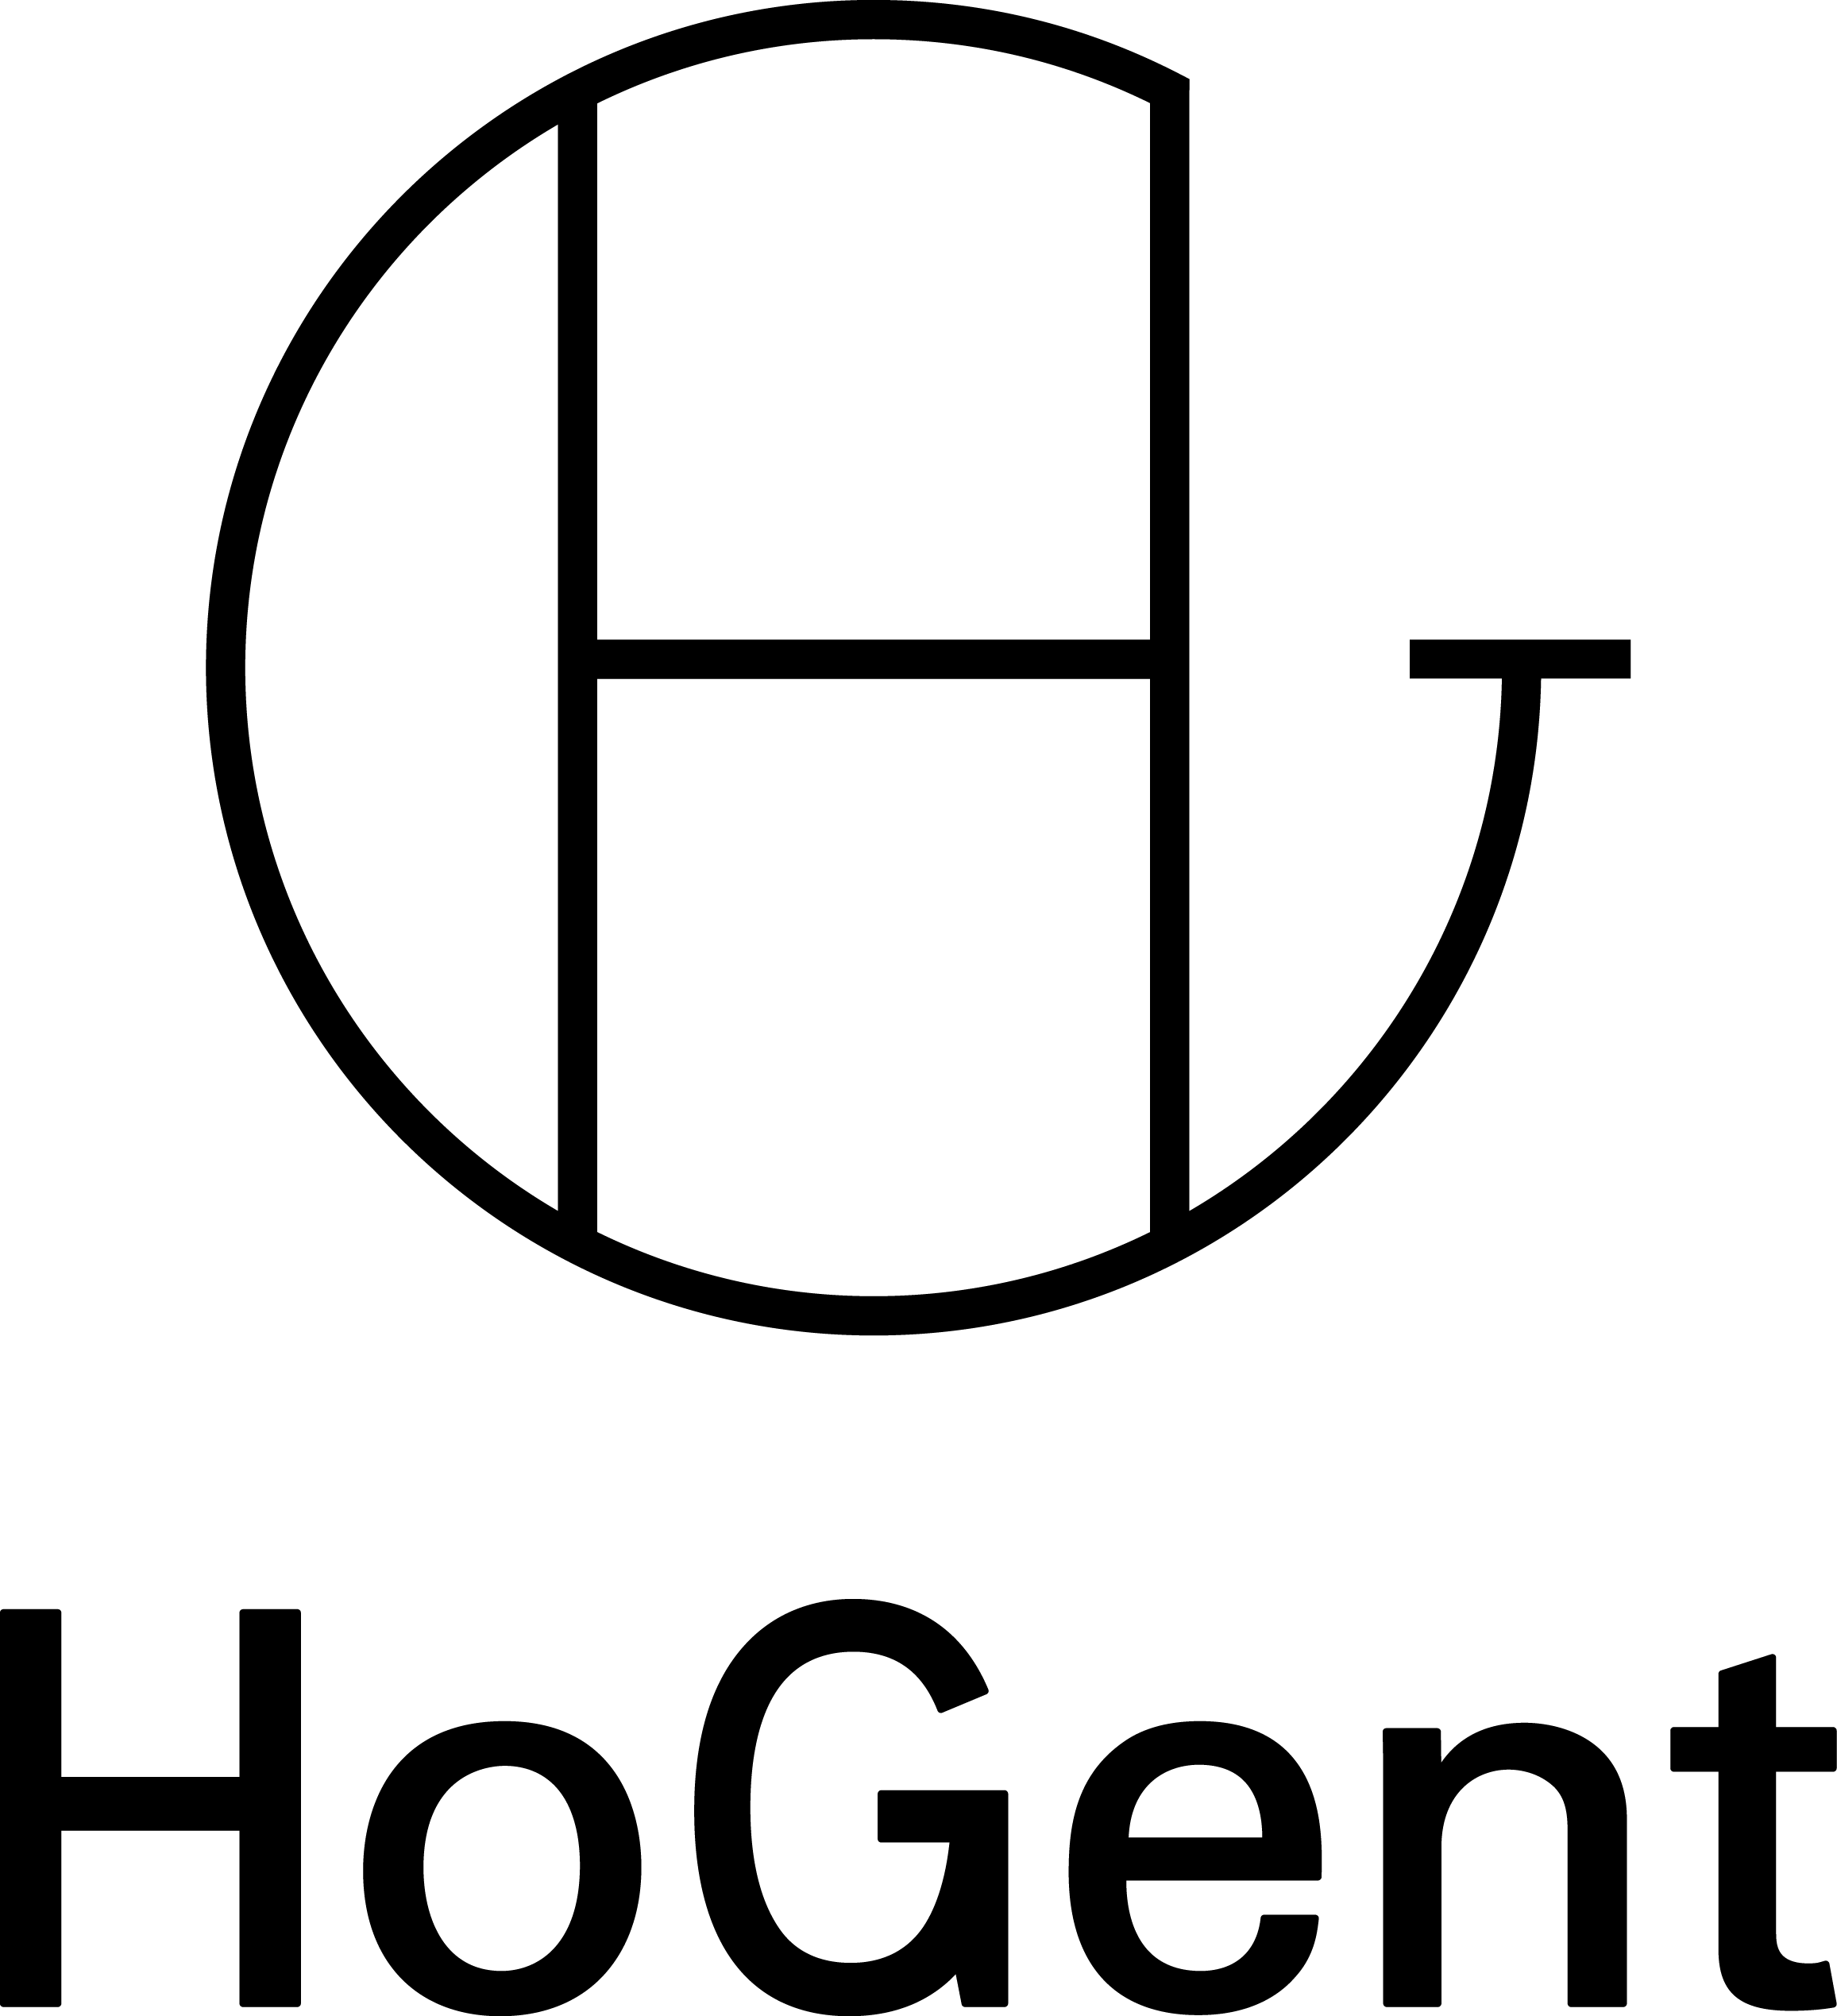
\includegraphics[width=2.5cm]{img/HG-beeldmerk-woordmerk}\\[.5cm]
    Faculteit Bedrijf en Organisatie\\[3cm]
    \titel
    \vfill
    \student\\[3.5cm]
    Scriptie voorgedragen tot het bekomen van de graad van\\professionele bachelor in de toegepaste informatica\\[2cm]
    Promotor:\\
    \promotor\\
    \ifdefempty{\copromotor}{\vspace{2.5cm}}{Co-promotor:\\\copromotor\\[2.5cm]}
    Instelling: \instelling\\[.5cm]
    Academiejaar: \academiejaar\\[.5cm]
    \ifcase \examenperiode \or Eerste \or Tweede \else Derde \fi examenperiode
    \endgroup

  \end{center}
  \restoregeometry
\end{titlepage}
  \emptypage
\begin{titlepage}
  \newgeometry{top=5.35cm,bottom=1.5cm,left=1.5cm,right=1.5cm}
  \begin{center}

    \begingroup
    \rmfamily
    \IfLanguageName{dutch}{Faculteit Bedrijf en Organisatie}{Faculty of Business and Information Management}\\[3cm]
    \titel
    \vfill
    \student\\[3.5cm]
    \IfLanguageName{dutch}{Scriptie voorgedragen tot het bekomen van de graad van\\professionele bachelor in de toegepaste informatica}{Thesis submitted in partial fulfilment of the requirements for the degree of\\professional bachelor of applied computer science}\\[2cm]
    Promotor:\\
    \promotor\\
    \ifdefempty{\copromotor}{\vspace{2.5cm}}{Co-promotor:\\\copromotor\\[2.5cm]}
    \IfLanguageName{dutch}{Instelling}{Institution}: \instelling\\[.5cm]
    \IfLanguageName{dutch}{Academiejaar}{Academic year}: \academiejaar\\[.5cm]
    \IfLanguageName{dutch}{%
    \ifcase \examenperiode \or Eerste \or Tweede \else Derde \fi examenperiode}{%
    \ifcase \examenperiode \or First \or Second \else Third \fi examination period}
    \endgroup

  \end{center}
  \restoregeometry
\end{titlepage}
}

%----------------------------------------------------------------------------------------
%	BIBLIOGRAPHY AND INDEX
%----------------------------------------------------------------------------------------

\usepackage[style=apa,backend=biber]{biblatex}
\usepackage{csquotes}
\DeclareLanguageMapping{dutch}{dutch-apa}
\addbibresource{bachproef-tin.bib} % BibTeX bibliography file
\defbibheading{bibempty}{}

\usepackage{calc} % For simpler calculation - used for spacing the index letter headings correctly
\usepackage{makeidx} % Required to make an index
\makeindex % Tells LaTeX to create the files required for indexing

%----------------------------------------------------------------------------------------
%	MAIN TABLE OF CONTENTS
%----------------------------------------------------------------------------------------

\usepackage{titletoc} % Required for manipulating the table of contents

\contentsmargin{0cm} % Removes the default margin

% Part text styling
\titlecontents{part}[0cm]
{\addvspace{20pt}\centering\large\bfseries}
{}
{}
{}

% Chapter text styling
\titlecontents{chapter}[1.25cm] % Indentation
{\addvspace{12pt}\large\sffamily\bfseries} % Spacing and font options for chapters
{\color{maincolor!60}\contentslabel[\Large\thecontentslabel]{1.25cm}\color{maincolor}} % Chapter number
{\color{maincolor}}
{\color{maincolor!60}\normalsize\;\titlerule*[.5pc]{.}\;\thecontentspage} % Page number

% Section text styling
\titlecontents{section}[1.25cm] % Indentation
{\addvspace{3pt}\sffamily\bfseries} % Spacing and font options for sections
{\contentslabel[\thecontentslabel]{1.25cm}} % Section number
{}
{\hfill\color{black}\thecontentspage} % Page number
[]

% Subsection text styling
\titlecontents{subsection}[1.25cm] % Indentation
{\addvspace{1pt}\sffamily\small} % Spacing and font options for subsections
{\contentslabel[\thecontentslabel]{1.25cm}} % Subsection number
{}
{\ \titlerule*[.5pc]{.}\;\thecontentspage} % Page number
[]

% List of figures
\titlecontents{figure}[0em]
{\addvspace{-5pt}\sffamily}
{\thecontentslabel\hspace*{1em}}
{}
{\ \titlerule*[.5pc]{.}\;\thecontentspage}
[]




% List of tables
\titlecontents{table}[0em]
{\addvspace{-5pt}\sffamily}
{\thecontentslabel\hspace*{1em}}
{}
{\ \titlerule*[.5pc]{.}\;\thecontentspage}
[]

%----------------------------------------------------------------------------------------
%	MINI TABLE OF CONTENTS IN PART HEADS
%----------------------------------------------------------------------------------------

% Chapter text styling
\titlecontents{lchapter}[0em] % Indenting
{\addvspace{15pt}\large\sffamily\bfseries} % Spacing and font options for chapters
{\color{maincolor}\contentslabel[\Large\thecontentslabel]{1.25cm}\color{maincolor}} % Chapter number
{}
{\color{maincolor}\normalsize\sffamily\bfseries\;\titlerule*[.5pc]{.}\;\thecontentspage} % Page number

% Section text styling
\titlecontents{lsection}[0em] % Indenting
{\sffamily\small} % Spacing and font options for sections
{\contentslabel[\thecontentslabel]{1.25cm}} % Section number
{}
{}

% Subsection text styling
\titlecontents{lsubsection}[.5em] % Indentation
{\normalfont\footnotesize\sffamily} % Font settings
{}
{}
{}

%----------------------------------------------------------------------------------------
%	PAGE HEADERS
%----------------------------------------------------------------------------------------

\usepackage{fancyhdr} % Required for header and footer configuration

\pagestyle{fancy}
\renewcommand{\chaptermark}[1]{\markboth{\sffamily\normalsize\bfseries\chaptername\ \thechapter.\ #1}{}} % Chapter text font settings
\renewcommand{\sectionmark}[1]{\markright{\sffamily\normalsize\thesection\hspace{5pt}#1}{}} % Section text font settings
\fancyhf{} \fancyhead[LE,RO]{\sffamily\normalsize\thepage} % Font setting for the page number in the header
\fancyhead[LO]{\rightmark} % Print the nearest section name on the left side of odd pages
\fancyhead[RE]{\leftmark} % Print the current chapter name on the right side of even pages
\renewcommand{\headrulewidth}{0.5pt} % Width of the rule under the header
\addtolength{\headheight}{2.5pt} % Increase the spacing around the header slightly
\renewcommand{\footrulewidth}{0pt} % Removes the rule in the footer
\fancypagestyle{plain}{\fancyhead{}\renewcommand{\headrulewidth}{0pt}} % Style for when a plain pagestyle is specified

% Removes the header from odd empty pages at the end of chapters
\makeatletter
\renewcommand{\cleardoublepage}{
\clearpage\ifodd\c@page\else
\hbox{}
\vspace*{\fill}
\thispagestyle{empty}
\newpage
\fi}

%----------------------------------------------------------------------------------------
%	THEOREM STYLES
%----------------------------------------------------------------------------------------

\usepackage{amsmath,amsfonts,amssymb,amsthm} % For math equations, theorems, symbols, etc

\newcommand{\intoo}[2]{\mathopen{]}#1\,;#2\mathclose{[}}
\newcommand{\ud}{\mathop{\mathrm{{}d}}\mathopen{}}
\newcommand{\intff}[2]{\mathopen{[}#1\,;#2\mathclose{]}}
\newtheorem{notation}{Notation}[chapter]

% Boxed/framed environments
\newtheoremstyle{maincolornumbox}% % Theorem style name
{0pt}% Space above
{0pt}% Space below
{\normalfont}% % Body font
{}% Indent amount
{\small\bf\sffamily\color{maincolor}}% % Theorem head font
{\;}% Punctuation after theorem head
{0.25em}% Space after theorem head
{\small\sffamily\color{maincolor}\thmname{#1}\nobreakspace\thmnumber{\@ifnotempty{#1}{}\@upn{#2}}% Theorem text (e.g. Theorem 2.1)
\thmnote{\nobreakspace\the\thm@notefont\sffamily\bfseries\color{black}---\nobreakspace#3.}} % Optional theorem note
\renewcommand{\qedsymbol}{$\blacksquare$}% Optional qed square

\newtheoremstyle{blacknumex}% Theorem style name
{5pt}% Space above
{5pt}% Space below
{\normalfont}% Body font
{} % Indent amount
{\small\bf\sffamily}% Theorem head font
{\;}% Punctuation after theorem head
{0.25em}% Space after theorem head
{\small\sffamily{\tiny\ensuremath{\blacksquare}}\nobreakspace\thmname{#1}\nobreakspace\thmnumber{\@ifnotempty{#1}{}\@upn{#2}}% Theorem text (e.g. Theorem 2.1)
\thmnote{\nobreakspace\the\thm@notefont\sffamily\bfseries---\nobreakspace#3.}}% Optional theorem note

\newtheoremstyle{blacknumbox} % Theorem style name
{0pt}% Space above
{0pt}% Space below
{\normalfont}% Body font
{}% Indent amount
{\small\bf\sffamily}% Theorem head font
{\;}% Punctuation after theorem head
{0.25em}% Space after theorem head
{\small\sffamily\thmname{#1}\nobreakspace\thmnumber{\@ifnotempty{#1}{}\@upn{#2}}% Theorem text (e.g. Theorem 2.1)
\thmnote{\nobreakspace\the\thm@notefont\sffamily\bfseries---\nobreakspace#3.}}% Optional theorem note

% Non-boxed/non-framed environments
\newtheoremstyle{maincolornum}% % Theorem style name
{5pt}% Space above
{5pt}% Space below
{\normalfont}% % Body font
{}% Indent amount
{\small\bf\sffamily\color{maincolor}}% % Theorem head font
{\;}% Punctuation after theorem head
{0.25em}% Space after theorem head
{\small\sffamily\color{maincolor}\thmname{#1}\nobreakspace\thmnumber{\@ifnotempty{#1}{}\@upn{#2}}% Theorem text (e.g. Theorem 2.1)
\thmnote{\nobreakspace\the\thm@notefont\sffamily\bfseries\color{black}---\nobreakspace#3.}} % Optional theorem note
\renewcommand{\qedsymbol}{$\blacksquare$}% Optional qed square
\makeatother

% Defines the theorem text style for each type of theorem to one of the three styles above
\newcounter{dummy}
\numberwithin{dummy}{section}
\theoremstyle{maincolornumbox}
\newtheorem{theoremeT}[dummy]{Theorem}
\newtheorem{problem}{Problem}[chapter]
\newtheorem{exerciseT}{Exercise}[chapter]
\theoremstyle{blacknumex}
\newtheorem{exampleT}{Example}[chapter]
\theoremstyle{blacknumbox}
\newtheorem{vocabulary}{Vocabulary}[chapter]
\newtheorem{definitionT}{Definition}[section]
\newtheorem{corollaryT}[dummy]{Corollary}
\theoremstyle{maincolornum}
\newtheorem{proposition}[dummy]{Proposition}

%----------------------------------------------------------------------------------------
%	DEFINITION OF COLORED BOXES
%----------------------------------------------------------------------------------------

\RequirePackage[framemethod=default]{mdframed} % Required for creating the theorem, definition, exercise and corollary boxes

% Theorem box
\newmdenv[skipabove=7pt,
skipbelow=7pt,
backgroundcolor=black!5,
linecolor=maincolor,
innerleftmargin=5pt,
innerrightmargin=5pt,
innertopmargin=5pt,
leftmargin=0cm,
rightmargin=0cm,
innerbottommargin=5pt]{tBox}

% Exercise box
\newmdenv[skipabove=7pt,
skipbelow=7pt,
rightline=false,
leftline=true,
topline=false,
bottomline=false,
backgroundcolor=maincolor!10,
linecolor=maincolor,
innerleftmargin=5pt,
innerrightmargin=5pt,
innertopmargin=5pt,
innerbottommargin=5pt,
leftmargin=0cm,
rightmargin=0cm,
linewidth=4pt]{eBox}

% Definition box
\newmdenv[skipabove=7pt,
skipbelow=7pt,
rightline=false,
leftline=true,
topline=false,
bottomline=false,
linecolor=maincolor,
innerleftmargin=5pt,
innerrightmargin=5pt,
innertopmargin=0pt,
leftmargin=0cm,
rightmargin=0cm,
linewidth=4pt,
innerbottommargin=0pt]{dBox}

% Corollary box
\newmdenv[skipabove=7pt,
skipbelow=7pt,
rightline=false,
leftline=true,
topline=false,
bottomline=false,
linecolor=gray,
backgroundcolor=black!5,
innerleftmargin=5pt,
innerrightmargin=5pt,
innertopmargin=5pt,
leftmargin=0cm,
rightmargin=0cm,
linewidth=4pt,
innerbottommargin=5pt]{cBox}

% Creates an environment for each type of theorem and assigns it a theorem text style from the "Theorem Styles" section above and a colored box from above
\newenvironment{theorem}{\begin{tBox}\begin{theoremeT}}{\end{theoremeT}\end{tBox}}
\newenvironment{exercise}{\begin{eBox}\begin{exerciseT}}{\hfill{\color{maincolor}\tiny\ensuremath{\blacksquare}}\end{exerciseT}\end{eBox}}
\newenvironment{definition}{\begin{dBox}\begin{definitionT}}{\end{definitionT}\end{dBox}}
\newenvironment{example}{\begin{exampleT}}{\hfill{\tiny\ensuremath{\blacksquare}}\end{exampleT}}
\newenvironment{corollary}{\begin{cBox}\begin{corollaryT}}{\end{corollaryT}\end{cBox}}

%----------------------------------------------------------------------------------------
%	REMARK ENVIRONMENT
%----------------------------------------------------------------------------------------

\newenvironment{remark}{\par\vspace{10pt}\small % Vertical white space above the remark and smaller font size
\begin{list}{}{
\leftmargin=35pt % Indentation on the left
\rightmargin=25pt}\item\ignorespaces % Indentation on the right
\makebox[-2.5pt]{\begin{tikzpicture}[overlay]
\node[draw=maincolor!60,line width=1pt,circle,fill=maincolor!25,font=\sffamily\bfseries,inner sep=2pt,outer sep=0pt] at (-15pt,0pt){\textcolor{maincolor}{R}};\end{tikzpicture}} % Orange R in a circle
\advance\baselineskip -1pt}{\end{list}\vskip5pt} % Tighter line spacing and white space after remark

%----------------------------------------------------------------------------------------
%	SECTION NUMBERING IN THE MARGIN
%----------------------------------------------------------------------------------------

\makeatletter
\renewcommand{\@seccntformat}[1]{\llap{\textcolor{maincolor}{\csname the#1\endcsname}\hspace{1em}}}
\renewcommand{\section}{\@startsection{section}{1}{\z@}
{-4ex \@plus -1ex \@minus -.4ex}
{1ex \@plus.2ex }
{\normalfont\large\sffamily\bfseries}}
\renewcommand{\subsection}{\@startsection {subsection}{2}{\z@}
{-3ex \@plus -0.1ex \@minus -.4ex}
{0.5ex \@plus.2ex }
{\normalfont\sffamily\bfseries}}
\renewcommand{\subsubsection}{\@startsection {subsubsection}{3}{\z@}
{-2ex \@plus -0.1ex \@minus -.2ex}
{.2ex \@plus.2ex }
{\normalfont\small\sffamily\bfseries}}
\renewcommand\paragraph{\@startsection{paragraph}{4}{\z@}
{-2ex \@plus-.2ex \@minus .2ex}
{.1ex}
{\normalfont\small\sffamily\bfseries}}

%----------------------------------------------------------------------------------------
%	PART HEADINGS
%----------------------------------------------------------------------------------------

% numbered part in the table of contents
\newcommand{\@mypartnumtocformat}[2]{%
\setlength\fboxsep{0pt}%
\noindent\colorbox{maincolor!20}{\strut\parbox[c][.7cm]{\ecart}{\color{maincolor!70}\Large\sffamily\bfseries\centering#1}}\hskip\esp\colorbox{maincolor!40}{\strut\parbox[c][.7cm]{\linewidth-\ecart-\esp}{\Large\sffamily\centering#2}}}%
%%%%%%%%%%%%%%%%%%%%%%%%%%%%%%%%%%
% unnumbered part in the table of contents
\newcommand{\@myparttocformat}[1]{%
\setlength\fboxsep{0pt}%
\noindent\colorbox{maincolor!40}{\strut\parbox[c][.7cm]{\linewidth}{\Large\sffamily\centering#1}}}%
%%%%%%%%%%%%%%%%%%%%%%%%%%%%%%%%%%
\newlength\esp
\setlength\esp{4pt}
\newlength\ecart
\setlength\ecart{1.2cm-\esp}
\newcommand{\thepartimage}{}%
\newcommand{\partimage}[1]{\renewcommand{\thepartimage}{#1}}%
\def\@part[#1]#2{%
\ifnum \c@secnumdepth >-2\relax%
\refstepcounter{part}%
\addcontentsline{toc}{part}{\texorpdfstring{\protect\@mypartnumtocformat{\thepart}{#1}}{\partname~\thepart\ ---\ #1}}
\else%
\addcontentsline{toc}{part}{\texorpdfstring{\protect\@myparttocformat{#1}}{#1}}%
\fi%
\startcontents%
\markboth{}{}%
{\thispagestyle{empty}%
\begin{tikzpicture}[remember picture,overlay]%
\node at (current page.north west){\begin{tikzpicture}[remember picture,overlay]%
\fill[maincolor!20](0cm,0cm) rectangle (\paperwidth,-\paperheight);
\node[anchor=north] at (4cm,-3.25cm){\color{maincolor!40}\fontsize{220}{100}\sffamily\bfseries\@Roman\c@part};
\node[anchor=south east] at (\paperwidth-1cm,-\paperheight+1cm){\parbox[t][][t]{8.5cm}{
\printcontents{l}{0}{\setcounter{tocdepth}{1}}%
}};
\node[anchor=north east] at (\paperwidth-1.5cm,-3.25cm){\parbox[t][][t]{15cm}{\strut\raggedleft\color{white}\fontsize{30}{30}\sffamily\bfseries#2}};
\end{tikzpicture}};
\end{tikzpicture}}%
\@endpart}
\def\@spart#1{%
\startcontents%
\phantomsection
{\thispagestyle{empty}%
\begin{tikzpicture}[remember picture,overlay]%
\node at (current page.north west){\begin{tikzpicture}[remember picture,overlay]%
\fill[maincolor!20](0cm,0cm) rectangle (\paperwidth,-\paperheight);
\node[anchor=north east] at (\paperwidth-1.5cm,-3.25cm){\parbox[t][][t]{15cm}{\strut\raggedleft\color{white}\fontsize{30}{30}\sffamily\bfseries#1}};
\end{tikzpicture}};
\end{tikzpicture}}
\addcontentsline{toc}{part}{\texorpdfstring{%
\setlength\fboxsep{0pt}%
\noindent\protect\colorbox{maincolor!40}{\strut\protect\parbox[c][.7cm]{\linewidth}{\Large\sffamily\protect\centering #1\quad\mbox{}}}}{#1}}%
\@endpart}
\def\@endpart{\vfil\newpage
\if@twoside
\if@openright
\null
\thispagestyle{empty}%
\newpage
\fi
\fi
\if@tempswa
\twocolumn
\fi}

%----------------------------------------------------------------------------------------
%	CHAPTER HEADINGS
%----------------------------------------------------------------------------------------

% A switch to conditionally include a picture, implemented by  Christian Hupfer
\newif\ifusechapterimage
\usechapterimagetrue
\newcommand{\thechapterimage}{}%
\newcommand{\chapterimage}[1]{\ifusechapterimage\renewcommand{\thechapterimage}{#1}\fi}%
\def\@makechapterhead#1{%
{\parindent \z@ \raggedright \normalfont
\ifnum \c@secnumdepth >\m@ne
\if@mainmatter
\begin{tikzpicture}[remember picture,overlay]
\node at (current page.north west)
{\begin{tikzpicture}[remember picture,overlay]
\node[anchor=north west,inner sep=0pt] at (0,0) {\ifusechapterimage\includegraphics[width=\paperwidth]{\thechapterimage}\fi};
\draw[anchor=west] (\Gm@lmargin,-9cm) node [line width=2pt,rounded corners=15pt,draw=maincolor,fill=white,fill opacity=0.5,inner sep=15pt]{\strut\makebox[22cm]{}};
\draw[anchor=west] (\Gm@lmargin+.3cm,-9cm) node {\huge\sffamily\bfseries\color{black}\thechapter. #1\strut};
\end{tikzpicture}};
\end{tikzpicture}
\else
\begin{tikzpicture}[remember picture,overlay]
\node at (current page.north west)
{\begin{tikzpicture}[remember picture,overlay]
\node[anchor=north west,inner sep=0pt] at (0,0) {\ifusechapterimage\includegraphics[width=\paperwidth]{\thechapterimage}\fi};
\draw[anchor=west] (\Gm@lmargin,-9cm) node [line width=2pt,rounded corners=15pt,draw=maincolor,fill=white,fill opacity=0.5,inner sep=15pt]{\strut\makebox[22cm]{}};
\draw[anchor=west] (\Gm@lmargin+.3cm,-9cm) node {\huge\sffamily\bfseries\color{black}#1\strut};
\end{tikzpicture}};
\end{tikzpicture}
\fi\fi\par\vspace*{270\p@}}}

%-------------------------------------------

\def\@makeschapterhead#1{%
\begin{tikzpicture}[remember picture,overlay]
\node at (current page.north west)
{\begin{tikzpicture}[remember picture,overlay]
\node[anchor=north west,inner sep=0pt] at (0,0) {\ifusechapterimage\includegraphics[width=\paperwidth]{\thechapterimage}\fi};
\draw[anchor=west] (\Gm@lmargin,-9cm) node [line width=2pt,rounded corners=15pt,draw=maincolor,fill=white,fill opacity=0.5,inner sep=15pt]{\strut\makebox[22cm]{}};
\draw[anchor=west] (\Gm@lmargin+.3cm,-9cm) node {\huge\sffamily\bfseries\color{black}#1\strut};
\end{tikzpicture}};
\end{tikzpicture}
\par\vspace*{270\p@}}
\makeatother

%----------------------------------------------------------------------------------------
%	HYPERLINKS IN THE DOCUMENTS
%----------------------------------------------------------------------------------------

\usepackage{hyperref}
\hypersetup{hidelinks,backref=true,pagebackref=true,hyperindex=true,colorlinks=false,breaklinks=true,urlcolor= maincolor,bookmarks=true,bookmarksopen=false,pdftitle={Title},pdfauthor={Author}}
\usepackage{bookmark}
\bookmarksetup{
open,
numbered,
addtohook={%
\ifnum\bookmarkget{level}=0 % chapter
\bookmarksetup{bold}%
\fi
\ifnum\bookmarkget{level}=-1 % part
\bookmarksetup{color=maincolor,bold}%
\fi
}
}

%----------------------------------------------------------------------------------------
%	Java source code
%----------------------------------------------------------------------------------------

% Commando voor invoegen Java-broncodebestanden (dank aan Niels Corneille)
% Gebruik:
%   \codefragment{source/MijnKlasse.java}{Uitleg bij de code}
%
% Je kan dit aanpassen aan de taal die je zelf het meeste gebruikt in je
% bachelorproef.
\newcommand{\codefragment}[2]{ \lstset{%
  language=java,
  breaklines=true,
  float=th,
  caption={#2},
  basicstyle=\scriptsize,
  frame=single,
  extendedchars=\true
}
\lstinputlisting{#1}}

% Leeg blad
\newcommand{\emptypage}{%
\newpage
\thispagestyle{empty}
\mbox{}
\newpage
}


%%---------- Documenteigenschappen --------------------------------------------
%% TODO: Vul dit aan met je eigen info:

% Je eigen naam
\newcommand{\student}{Yannick Servranckx}

% De naam van je promotor (lector van de opleiding)
\newcommand{\promotor}{Lotte Van Steenberghe}

% De naam van je co-promotor. Als je promotor ook je opdrachtgever is en je
% dus ook inhoudelijk begeleidt (en enkel dan!), mag je dit leeg laten.
\newcommand{\copromotor}{}

% Indien je bachelorproef in opdracht van/in samenwerking met een bedrijf of
% externe organisatie geschreven is, geef je hier de naam. Zoniet laat je dit
% zoals het is.
\newcommand{\instelling}{---}

% De titel van het rapport/bachelorproef
\newcommand{\titel}{Progressive webapp}

% Datum van indienen (gebruik telkens de deadline, ook al geef je eerder af)
\newcommand{\datum}{27 mei 2016}

% Academiejaar
\newcommand{\academiejaar}{2017-2018}

% Examenperiode
%  - 1e semester = 1e examenperiode => 1
%  - 2e semester = 2e examenperiode => 2
%  - tweede zit  = 3e examenperiode => 3
\newcommand{\examenperiode}{3}

%%=============================================================================
%% Inhoud document
%%=============================================================================

\begin{document}

%---------- Taalselectie ------------------------------------------------------
%% Als je je bachelorproef in het Engels schrijft, haal dan onderstaande regel
%% uit commentaar. Let op: de tekst op de voorkaft blijft in het Nederlands, en
%% dat is ook de bedoeling!
%\selectlanguage{english}

%---------- Titelblad ---------------------------------------------------------
\inserttitlepage

%---------- Samenvatting, voorwoord -------------------------------------------
\usechapterimagefalse
%%=============================================================================
%% Samenvatting
%%=============================================================================

%% TODO: De "abstract" of samenvatting is een kernachtige (~ 1 blz. voor een
%% thesis) synthese van het document.
%%
%% Deze aspecten moeten zeker aan bod komen:
%% - Context: waarom is dit werk belangrijk?
%% - Nood: waarom moest dit onderzocht worden?
%% - Taak: wat heb je precies gedaan?
%% - Object: wat staat in dit document geschreven?
%% - Resultaat: wat was het resultaat?
%% - Conclusie: wat is/zijn de belangrijkste conclusie(s)?
%% - Perspectief: blijven er nog vragen open die in de toekomst nog kunnen
%%    onderzocht worden? Wat is een mogelijk vervolg voor jouw onderzoek?
%%
%% LET OP! Een samenvatting is GEEN voorwoord!



\chapter*{\IfLanguageName{dutch}{Samenvatting}{Abstract}}

Tot hoe laat was de winkel weer open? Snel even mijn gsm pakken en naar de openingsuren kijken. Steeds meer en meer worden websites mobiel geopend in plaats van op desktop/laptop. Als bedrijf is het dan ook belangrijk dat men hierop inspeelt en zorgt dat hun gebruikers altijd en overal bij hen terecht kunnen.
Hoe ga je als bedrijf hier mee om? Ga je voor een klassieke website die gebruikers zowel mobiel als op hun laptop kunnen bezoeken en die makkelijk kan gedeeld worden via een link? Of laat je de site achterwege en ga je voor een mobiele app? 

Als bedrijf is het belangrijk te onderzoeken wat je klanten willen en op welke manier ze jouw product zoveel mogelijk gaan gebruiken. Wil je hen de app laten installeren, waarop veel mensen al zullen afhaken, zodat ze je app steeds makkelijk kunnen openen of wil je hen steeds laten terugsurfen naar je site? Door dit te onderzoeken kan je kijken op welke manier je product bij zoveel mogelijk klanten komt en kun je je hier eventueel aan aanpassen. 

Native apps en web apps zijn twee verschillende types van applicaties. Native apps zijn specifiek voor elk platform. Voor zowel Apple, Android of Windows is er een andere programmeertaal nodig. Ze worden speciaal voor een bepaald platform ontwikkeld. Daardoor hebben ze verschillende functionaliteiten van een apparaat die ze kunnen gebruiken, zoals de camera, die een web app niet kan. Web apps daarentegen zijn platform onafhankelijk hierdoor hoeven ze maar eenmaal ontwikkeld te worden en kunnen direct op alle platformen bekeken worden. Web apps draaien op een browser en zijn meestal geschreven in HTML5. 

Zowel het web als native apps hebben voor- en nadelen. Er was dus nood aan iets dat deze twee kon combineren en dit iets is progressive web apps. Door gebruik van service worker, een app shell en web app manifest, lijkt en gedraagt een progressive web app zich als een native app. Aangezien progressive web apps een web app is kan deze op alle platformen draaien en hoeft het slechts eenmaal ontwikkeld te worden. 

Het hoofddoel van deze thesis was het onderzoeken en implementeren van een progressive web app en te bekijken wat de belangrijkste onderdelen hiervan zijn. Hiervoor heb ik een progressive web app ontwikkeld die gaat belichten op welke manier een progressive web app een native als een web app combineert. Hiernaast heb ik ook gekeken wat de voor- en nadelen van een progressive web app zijn en deze vergeleken met een native app.

Een progressive web app heeft veel voordelen tegenover een standaard web app en is voor het web een grote stap vooruit. Het web groeit en zal altijd blijven groeien. Het is belangrijk als bedrijf hierop in te spelen. Je kan een nieuwe webapp maken en deze direct volledig als progressive web app maken. Het voordeel is dat je een huidge web app progressief kan omzetten naar een progressive web app. Je voegt enkel de functionaliteiten toe die je zelf wil of nodig hebt. Als eigenaar van een web app is het dus belangrijk te kijken welke mogelijkheden je hebt om eventueel één of meerdere functionaliteiten toe te voegen. Dit zal je web app enkel positief beïnvloeden. 

Ondanks de verscheidene voordelen van een progressive web app tegenover een native app zal de web app nog niet direct de native app verdrijven van onze mobiele apparaten. Toch zullen progressive web apps steeds meer gebruikt worden en ingeburgerd raken, waardoor dit toch wel een vast gegeven zal worden in de toekomst van onze mobiele apparaten.






%%=============================================================================
%% Voorwoord
%%=============================================================================

\chapter*{Voorwoord}
\label{ch:voorwoord}

%% TODO:
%% Het voorwoord is het enige deel van de bachelorproef waar je vanuit je
%% eigen standpunt (``ik-vorm'') mag schrijven. Je kan hier bv. motiveren
%% waarom jij het onderwerp wil bespreken.
%% Vergeet ook niet te bedanken wie je geholpen/gesteund/... heeft

Deze bachelorproef is tot stand gekomen in het kader van het behalen van het diploma Bachelor in Toegepaste Informatica.

Aangezien ik altijd veel interesse had in native apps heb ik voor progressive web apps als onderwerp gekozen. Native apps leek me altijd een groot voordeel te hebben tegenover web apps. Toen ik voor het eerst hoorde van progressive web apps leek dit me direct interessant aangezien dit het beste van twee werelden combineert. Misschien was dit wel de opvolger van native apps. Het was het dus zeker waard om dit eens beter te onderzoeken.

Een woord van dank aan mijn promotors Lotte Van Steenberghe en Johan Decorte. Mede dankzij hun feedback heb ik deze bachelorproef tot een goed einde kunnen brengen.

Daarnaast wil ik ook mijn vriendin, Devette Garza, bedanken om mij altijd aan te moedigen en in mij te blijven geloven.

Tot slot wil ik ook Thibault de Gryse en Ingrid De Keyser bedanken voor het nalezen van mijn eindwerk en me te ondersteunen waar nodig.


%---------- Inhoudstafel ------------------------------------------------------
\pagestyle{empty} % No headers
\tableofcontents % Print the table of contents itself
\cleardoublepage % Forces the first chapter to start on an odd page so it's on the right
\pagestyle{fancy} % Print headers again

%---------- Lijst afkortingen, termen -----------------------------------------
%% Als je een lijst van afkortingen of termen wil toevoegen, dan hoort die
%% hier thuis. Gebruik bijvoorbeeld de ``glossaries'' package.

%%---------- Kern -------------------------------------------------------------


%%=============================================================================
%% Inleiding
%%=============================================================================

\chapter{Inleiding}
\label{ch:inleiding}

\nocite{*}

“The full Safari engine is inside of iPhone. And so, you can write amazing Web 2.0 and Ajax apps that look exactly and behave exactly like apps on the iPhone. And these apps can integrate perfectly with iPhone services. They can make a call, they can send an email, they can look up a location on Google Maps. And guess what there is no SKD that you need. You got everything you need if you know how to write apps using the most modern web standards to write amazing apps for the IPhone today” ~\autocite{keynote2007}

Steve Jobs schetste in zijn speech in 2007 al een idee omtrent wat we tegenwoordig progressive web apps ofwel PWA's noemen. Hierbij stelde hij Apple's internetbrowser Safari voor, waarop hij een idee gaf wat er allemaal mogelijk mee is. In 2008 introduceerde Apple de App Store waardoor het idee rond progressive web apps meer op de achtergrond raakte.

De voorbije jaren zijn er drie grote spelers op de mobiele markt geweest. Apple, Windows en Android. Elk van deze hebben hun eigen store waar ze apps aanbieden en waar je als ontwikkelaar je apps op kunt lanceren. Elke store werkt met een eigen programmeertaal.
\begin{itemize}  
	\item Android: Java
	\item Apple: Recent overgeschakeld van Objective-C naar Swift
	\item Windows: C\#
\end{itemize}

Je hoeft je app niet op de store te plaatsen. Je kan dit ook aanbieden op je eigen website. Hiervoor moeten gebruikers je APK downloaden en installeren. Een 'Android Package Kit' of APK is de bestandsextensie die gebruikt wordt door het besturingssysteem van Android voor hun mobiele apps. Net zoals Windows .exe bestanden heeft, gebruikt Android .apk ~\autocite{apk}

Als ontwikkelaar wil je geen drie verschillende programmeertalen leren. Als bedrijf wil je niet drie verschillende mensen huren voor hetzelfde werk te doen.

Op de Google I/O developer conference heeft Google als antwoord hierop de progressive web app voorgesteld. Google beschrijft de progressive web app als 'applicaties die gebruik maken van nieuwe technologieën om zo het beste van native apps en mobiele website naar de gebruiker te brengen. Ze zijn betrouwbaar en snel'.
Met andere woorden: Google wil webapplicaties die de voordelen van native apps gaan gebruiken zodat de webapp zich gaat gedragen als een native app. 
Als ontwikkelaar zou je dan eenmaal je webapp moeten maken en kan deze op eender welk platform bekeken en gebruikt worden. Je zou geen verschillende programmeertalen moeten leren om dit voor elk platform apart te maken en toch zal het op elk platform lijken alsof het een native app is, speciaal gemaakt voor Android, Apple ...






\section{Stand van zaken}
\label{sec:stand-van-zaken}

%% TODO: deze sectie (die je kan opsplitsen in verschillende secties) bevat je
%% literatuurstudie. Vergeet niet telkens je bronnen te vermelden!
Voordat we kunnen gaan kijken wat nu het beste alternatief is moeten we eerst begrijpen wat nu juist een PWA is en wat een native app is.

\subsection{Wat is een native app?}
Een native mobile app is een applicatie voor op de smartphone die gemaakt is voor gebruik op een specifiek platform in een specifieke programmeertaal ~\autocite{mobileWat}. Doordat een app specifiek voor dat platform gemaakt is, kan de app gebruik maken van enkele interne technologieën van de smartphone zoals GPS, bluetooth, camera... Een goed voorbeeld hierbij is Pokemon Go. Pokemon Go maakt gebruik van vele verschillende functionaliteiten van je smartphone. Het gaat je camera gebruiken voor de Pokemons weer te geven in de echte wereld, je GPS gebruiken om te weten waar je bent, meten hoe snel je gaat ...  Doordat Pokemon Go een native app is die speciaal gemaakt is voor het platform waarop het draait, dit kan zowel Apple als Android zijn, krijgt het de mogelijkheid om deze functionaliteiten te gebruiken. 

Een ontwikkelaar die een native app maakt gaat afhankelijk van het platform een andere programmeertaal moeten gebruiken. Eenmaal zijn app geschreven is kan hij deze door gebruikers laten downloaden. Hij kan dit aanbieden op zijn eigen site via de APK ofwel via de store. Na installatie worden gegevens op de mobiele telefoon opgeslagen. De gebruiker kan nadien de app gebruiken zonder deze opnieuw te moeten installaren. (zie overzicht \ref{table:webVsNative}).


% first column
\begin{minipage}[t]{0.5\textwidth}
	\textbf{Voordelen}
	\begin{itemize}  
		\item Maximaal gebruik van alle functionaliteiten van het apparaat (camera, GPS, \dots)
		\item Geen internetverbinding nodig
		\item Integratiemogelijkheden met andere apps
		\item Hogere snelheid op het apparaat
	\end{itemize}
\end{minipage}
%second column
\begin{minipage}[t]{0.5\textwidth}
		\textbf{Nadelen}
	\begin{itemize}  
		\item Per platform moet apart ontwikkeld worden
		\item Goedkeuring voor plaatsing in de store
		\item Updates in software van het platform (bv. na een update van Android) is het mogelijk dat de app moet worden aangepast
\end{itemize}
\end{minipage}


\subsection{Wat is een web app?}
Steeds meer worden websites mobiel bezocht. In 2017 werden 37\% van de websites bezocht via desktop en 63\% mobiel.(\ref{fig:visitsWeb}) Gebaseerd op deze gegevens lijkt het waarschijnlijk dat aan het einde van 2018 66\% van alle bezoeken op websites via de mobiele telefoon zal zijn.~\autocite{traffic}. Hierdoor is het dus belangrijk dat je je website optimaliseert voor mobiel gebruik. Een website die hiervoor is geoptimaliseerd is een webapp. Webapps moeten altijd bezocht worden via de browser. De gebruiker gaat naar zijn favoriete internetbrowser en kan via de link de webapp opzoeken en bezoeken. Webapps hoeven dus niet geïnstalleerd te worden. Met behulp van een bladwijzer kan een koppeling gemaakt worden op het home-scherm van je apparaat. (zie overzicht \ref{table:webVsNative}).


% first column
\begin{minipage}[t]{0.5\textwidth}
	\textbf{Voordelen}
	\begin{itemize}  
		\item Doordat het een webapp is, is het niet platformafhankelijk. 
		\item Makkelijk te delen. Je deelt gewoon een link en de gebruiker moet niets installeren
		\item Gebruikers zien altijd de laatste versie zonder updates te hoeven downloaden van de app.
	\end{itemize}
\end{minipage}
%second column
\begin{minipage}[t]{0.5\textwidth}
	\textbf{Nadelen}
	\begin{itemize}  
		\item Het kan niet alle functionaliteiten van je apparaat gebruiken
		\item Een webapp is niet vindbaar in de store
	\end{itemize}
\end{minipage}


\subsection{Web vs Native}
Uit een onderzoek van \textcite{comScore} in 2016 is gebleken  dat gebruikers 87\% van hun tijd op de smarthphone of tablet doorbrengen op een mobiele app terwijl ze maar 13\% van hun tijd doorbrengen op het web. Als je deze cijfers ziet, zou je je kunnen afvragen of het wel slim is je tijd te investeren in een web app. Is het niet beter je tijd te spenderen aan het ontwikkelen van native apps? Je hebt wat meer werk om het op elk platform apart te kunnen krijgen, maar als je cijfers ziet van de gebruikers lijkt het erop dat het wel zijn vruchten kan afwerpen.
(zie figuur \ref{fig:usage}). 

Ondanks dat de gebruiker gemiddeld meer tijd doorbrengt op een native app zien we in hetzelfde onderzoek van \textcite{comScore}  dat de helft van alle gebruikers maar 1 app per maand downloadt. Dit is een zeer laag nummer als je weet dat er in het eerste kwartaal van 2018 ongeveer 7.133.500 apps beschikbaar waren over de verschillende stores. Als je enkel kijkt naar degenen die wel apps downloaden merk je dat deze gemiddeld 3,5 apps per maand downloaden. Meer dan de helft van deze apps wordt gedownload door 13\% van de smartphone eigenaars. (zie figuur \ref{fig:downloads}).

Ondanks dat gebruikers meer tijd spenderen op apps dan op mobiele websites, zijn er maandelijks meer unieke gebruikers die gebruik maken van een website dan van een app. (zie figuur \ref{fig:visitors} ) Hieruit kunnen we concluderen dat gebruikers weliswaar meer tijd doorbrengen op apps, maar dat ze wel online actiever bezig zijn. Gebruikers gaan niet zoveel nieuwe apps downloaden, maar wel veel tijd doorbrengen op hun favoriete app. Gemiddeld brengen gebruikers 45\% van hun tijd door op hun favoriete app en 75\% met hun top 3 apps (zie figuur \ref{fig:timeSpent}).

Als je een native app hebt, heb je veel concurrenten. Het is moeilijk om veel gebruikers te krijgen aangezien maar weinigen nieuwe apps downloaden. Toch zijn de gebruikers loyaal aan hun favoriete apps en spenderen ze er veel tijd aan.


\subsection{PWA's}
Een progressive web app gaat nog een stap verder. Een progressive web app is een web app die er net als een native app uitziet en zich net zoals een native app gaat gedragen. Als gebruiker kun je de app installeren op je apparaat waardoor je een snelkoppeling krijgt. De app zal ook offline gebruikt kunnen worden. Omdat het nog steeds een webapp is kan je deze gewoon via je internetbrowser vinden. Maar vanaf wanneer is je webapp een progressive web app? 

Progressive web apps worden niet in een bepaalde code geschreven. Je kan elke (bestaande) webapp gaan aanpassen zodat ze progressief is. Dit hoef je niet in een keer te doen. Je gaat de functionaliteiten gaan implementeren die je wil of nodig hebt. Indien je later andere functionaliteiten hebt, kan je deze dan gaan toevoegen.
Enkele belangrijke kenmerken van een progressive webapp zijn:

\begin{itemize}  
	\item Progressief: \\
	Een progressive webapp moet werken voor alle gebruikers, op elke browser, op elk platform en gebruik maken van de functionaliteiten van het apparaat. Hierbij zullen sommige browsers of nieuwere versies meer functionaliteiten aanbieden dan andere. Het is de bedoeling dat alles goed werkt, ook als je browser bepaalde functionaliteiten niet ondersteunt die je in je app gebruikt. \\ 
	\item Responsief: \\
	Een progressive webapp moet geschikt zijn voor elk apparaat, welk grootte ook. Of je webapp nu bezocht wordt op een klein scherm van je telefoon of op het scherm van je desktop, overal moet de kwaliteit van je app even goed zijn. 
	\\
	\item Installeerbaar: \\
	Je kan een sneltoets opslaan op je home screen. Hierdoor kan de gebruiker met één klik terug naar de app navigeren.
	\\
	\item Gedraagt zich als native app: \\
	Wanneer je de app opent via de sneltoets gaat de progressive web app eruit zien als een native app ondanks dat dit nog steeds een webapp is.
	\\
	\item Onafhankelijk van internet: \\
	Een progressive web app kan met een slecht netwerk of volledig offline werken. Door het opslaan van bestanden op het apparaat zelf, ook wel cachen genoemd, kan de app offline blijven werken. Bij een slechte internetverbinding kan hij deze bestanden ook gebruiken zodat de gebruiker geen wachttijden heeft. Het verliezen van connectiviteit is geen probleem, maar een mogelijkheid en moet daarom zeer zorgvuldig worden opgevangen. De ontwikkelaar moet daarom zien dat zodra er internetconnectie is, bestanden steeds up-to-date zijn zodat een gebruiker nooit oude data ziet.
	\\
		\item Ontdekbaar: \\
	Dankzij het W3C-manifest is het identificeerbaar als app en kan het gevonden worden door zoekmachines
	\\
		\item Deelbaar: \\
	Je kan makkelijk een link delen zodat anderen je applicatie kunnen bekijken. Installatie is niet nodig.
	\\
		\item Veilig: \\
	Progressive web apps gebruiken een beveiligde HTTPS-verbinding zodat alle data veilig kan worden uitgewisseld.
	\\
		\item Push notificaties \\
	Je kan push notificaties sturen naar de gebruikers. Dit verhoogt de kans dat gebruikers terug keren naar je app. De push notificaties voelen aan als notificaties van echte apps.
	\\
\end{itemize}





\section{Probleemstelling en Onderzoeksvragen}
\label{sec:onderzoeksvragen}

%% TODO:
%% Uit je probleemstelling moet duidelijk zijn dat je onderzoek een meerwaarde
%% heeft voor een concrete doelgroep (bv. een bedrijf).
%%
%% Wees zo concreet mogelijk bij het formuleren van je
%% onderzoeksvra(a)g(en). Een onderzoeksvraag is trouwens iets waar nog
%% niemand op dit moment een antwoord heeft (voor zover je kan nagaan).

Als bedrijf wil je gemakkelijk gevonden worden door iedereen. Wat voor bedrijf je ook hebt, of je nu spelletjes maakt online, of je nu een bakkerij hebt of een groentenwinkel, een groot bedrijf met honderden werknemers of een eenmanszaak. Als potentiële klanten iets zoeken wat jij aanbiedt, dan wil je snel en eenvoudig gevonden worden. Maar hoe kan je dit het best doen? 

Hulpvragen:
\begin{itemize}  
	\item Investeer je als bedrijf het beste in native of in progressive web apps?
\end{itemize}



\section{Opzet van deze bachelorproef}
\label{sec:opzet-bachelorproef}

%% TODO: Het is gebruikelijk aan het einde van de inleiding een overzicht te
%% geven van de opbouw van de rest van de tekst. Deze sectie bevat al een aanzet
%% die je kan aanvullen/aanpassen in functie van je eigen tekst.

De rest van deze bachelorproef is als volgt opgebouwd:

In hoofdstuk~\ref{ch:methodologie} wordt de methodologie toegelicht en worden de gebruikte onderzoekstechnieken besproken om een antwoord te kunnen formuleren op de onderzoeksvragen.

%% TODO: Vul hier aan voor je eigen hoofstukken, één of twee zinnen per hoofdstuk

In hoofdstuk~\ref{ch:conclusie}, tenslotte, wordt de conclusie gegeven en een antwoord geformuleerd op de onderzoeksvragen. Daarbij wordt ook een aanzet gegeven voor toekomstig onderzoek binnen dit domein.


%%=============================================================================
%% Methodologie
%%=============================================================================

\chapter{Methodologie}
\label{ch:methodologie}

%% TODO: Hoe ben je te werk gegaan? Verdeel je onderzoek in grote fasen, en
%% licht in elke fase toe welke stappen je gevolgd hebt. Verantwoord waarom je
%% op deze manier te werk gegaan bent. Je moet kunnen aantonen dat je de best
%% mogelijke manier toegepast hebt om een antwoord te vinden op de
%% onderzoeksvraag.

\section{PWA Componenten}
Om een progressive web app te maken zijn er enkele belangrijke componenten. Deze gaan er voor zorgen dat je een optimale user experience krijgt net zoals je een native app zou hebben.
\begin{itemize}  
	\item Application shell
	\item Web App Manifest
	\item Service Worker
\end{itemize}

\subsection{Web App Manifest}
\lstset{
	string=[s]{"}{"},
	stringstyle=\color{blue},
	comment=[l]{:},
	commentstyle=\color{black},
}
Je web app manifest is een simpel JSON bestand waarin je aan de browser vertelt over je web app en hoe het zich moet gedragen als het geïnstalleerd wordt op het apparaat van de gebruiker. Zonder dit manifest zal Chrome nooit de optie geven aan de gebruiker om de app te installeren op het hoofdscherm (zie figuur \ref{fig:promptHome} ) \\

Een typisch manifest ziet er als volgt uit: 
	\begin{lstlisting}
{
"name": "Instagram als Progressive Web App",
"short_name": "PWAGram",
"icons": [
{
"src": "/src/images/icons/app-icon-48x48.png",
"type": "image/png",
"sizes": "48x48"
},
{
"src": "/src/images/icons/app-icon-96x96.png",
"type": "image/png",
"sizes": "96x96"
},
{
"src": "/src/images/icons/app-icon-144x144.png",
"type": "image/png",
"sizes": "144x144"
},
{
"src": "/src/images/icons/app-icon-192x192.png",
"type": "image/png",
"sizes": "192x192"
},
{
"src": "/src/images/icons/app-icon-256x256.png",
"type": "image/png",
"sizes": "256x256"
},
{
"src": "/src/images/icons/app-icon-384x384.png",
"type": "image/png",
"sizes": "384x384"
},
{
"src": "/src/images/icons/app-icon-512x512.png",
"type": "image/png",
"sizes": "512x512"
}
],
"start_url": "/index.html",
"scope": ".",
"display": "standalone",
"orientation": "portrait-primary",
"background_color": "#fff",
"theme_color": "#3f51b5",
"description": "Een simpele Instagram Clone.",
"dir": "ltr",
"lang": "nl-BE"
}
\end{lstlisting}


\clearpage
\begin{itemize}  
	\item name en short\_name: \\
	Eén van deze twee moet zeker aanwezig zijn. Als beide voorzien zijn zal overal de short\_name gebruikt worden waar de plaats beperkt is zoals op je hoofdscherm onder het icoon.
	\\
	\item icons \\
	Hier kun je je iconen definiëren. Je definiëert een lijst met je iconen. De browser zal dan de beste uitpakken voor hetgeen nodig is. Als de browser het icoon nodig heeft voor te tonen op je hoofdscherm zal hij hier hetgeen met de juiste afmetingen bepalen.
	\\
	\item start\_url: \\
	Dit vertelt aan de browser welke startpagina getoond moet worden aan de gebruiker. 
	\\
	\item scope: \\
	Welke pagina's zijn deel van de progressive web app en kunnen dus gebruik maken van de iconen en kleuren die zijn gedefiniëerd. Het is gebruikelijk om hier alle pagina's te kiezen. Dit kan door gewoon "." te zetten. 
	\\

	\item display: \\
	Hier kun je specifiëren welk deel van de browser getoond moet worden. Je kan aan de gebruiker nog steeds de adresbar tonen of je kan ervoor kiezen om alles te verbergen zodat het meer als een native app aanvoelt. \\
	\bigbreak
	\begin{longtable}
		\begin{tabular}{| p{.20\textwidth} | p{.80\textwidth} |}
			\hline
			\textbf{Waardes} & \textbf{Beschrijving} & & \\
			\hline
		
			 \textbf{fullscreen} & Neemt het geheel van plaats in beslag op het scherm en toont geen andere elementen. &  &  \\ 
			\hline
			\textbf{standalone} & De webapp zal eruit zien als een echte native app. Het opent op een apart venster, apart van de browser en toont geen standaard browser elementen zoals de zoekbalk. &  &  \\
			\hline
			\textbf{minimal-ui} & Dit wordt niet ondersteund in chrome. Hierbij heb je net hetzelfde als bij fullscreen maar je hebt een minimaal aantal aan elementen die je kan zien zoals een back-knop. &  &  \\
			\hline
			 \textbf{browser} & Het lijkt alsof je gewoon in de browser kijkt. &  & \\
			\hline
		\end{tabular}
	\end{longtable}

	\item background\_color: \\
De achtergrondkleur van de app. Dit wordt vooral getoond in laadschermen. Hiervoor gebruik je een hexadecimale code bv: #fff
\\


	\item theme\_color: \\
	Je thema kleur. Net zoals native apps een thema kleur hebben die gaat bepalen welke kleur je balk aan de top van je scherm heeft. Ook hier wordt gebruik gemaakt van een hexadecimale code
	\\
	\item description: \\
	Hier kan je een kleine samenvatting geven. Als een internetbrowser dit nodig heeft, zal hij dit hier vandaan halen. De gebruiker zal dit dus te zien krijgen.	
	\\
	\item dir \\
	Dit is de richting van je tekst. Doorgaans wordt hier ltr gebruikt, left to right. Als je wil kan je hier ook rtl kiezen.
	\\
	\item lang \\
	De taal van je app: je gebruikt hier de 4 letter code van de taal die je wil.
	\\
	\item orientation \\
	Hier kan je bepalen hoe je wil dat je app getoond wordt. Wil je dit rechtop of liever gedraaid. Je kan hier aan de gebruiker opleggen dat je het scherm niet kunt draaien. vb: portrait-primary
	\\
	
\end{itemize}


Na het toevoegen van je manifest moet je aan al je pagina's de link naar je manifest toevoegen.
\begin{lstlisting}
<link rel="manifest" href="/manifest.json">
\end{lstlisting}

Nadien kan je je manifest controleren in de developer tools van Google Chrome


	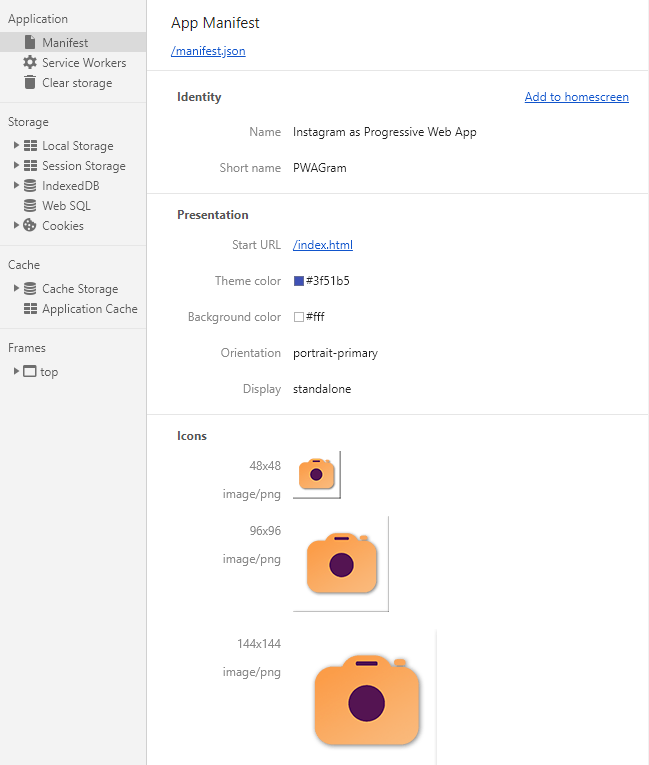
\includegraphics[scale=0.5]{img/manifestDev.png}



\subsection{Service Worker}
Het web is handig. Wil je de openingsuren van een winkel weten of wil je opzoeken wat ze allemaal verkopen? Ga naar hun website en je vindt het meteen. Het is zo makkelijk. En toch heeft iedereen al eens hetzelfde meegemaakt als ze dit willen doen: \\

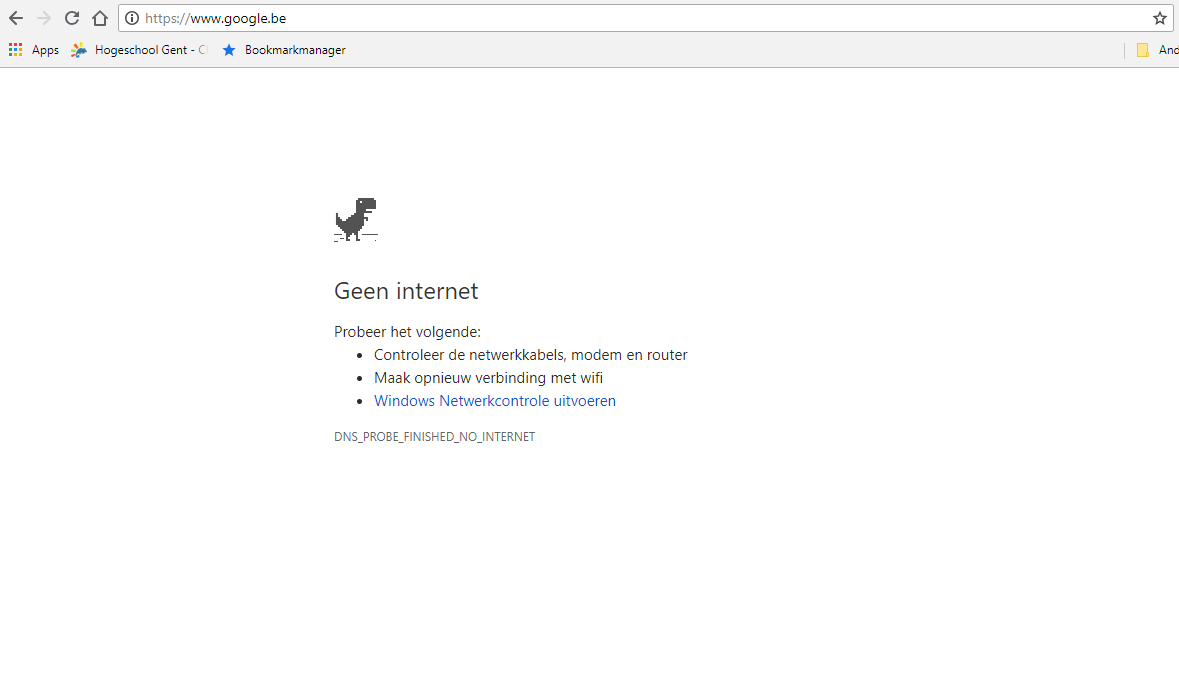
\includegraphics[scale=0.5]{img/noInternet.png}


Zoals je ziet kun je niet veel zien als je geen internet hebt. Zonder internet kan je niet de informatie gaan opzoeken die je nodig hebt.

Door de introductie van de service worker is dit voor ontwikkelaars niet langer een probleem en kunnen ze dit op een juiste manier verwerken zodat de gebruikers niet merken dat ze geen internet hebben. Dit is de belangrijkste taak van de service worker maar lang niet de enige.

Een service worker is een script dat, apart van de webpagina, op de browser draait. Hierdoor zijn er verschillende functionaliteiten die gebruikt kunnen worden waarbij geen interactie van de gebruiker nodig is. Momenteel zijn dit functionaliteiten zoals push notificaties of offline gebruik van de site maar wie weet welke functionaliteiten in de toekomst nog mogelijk zullen worden gemaakt. 


Aangezien een service worker apart loopt van de webpagina heeft het ook een andere levenscyclus. 

	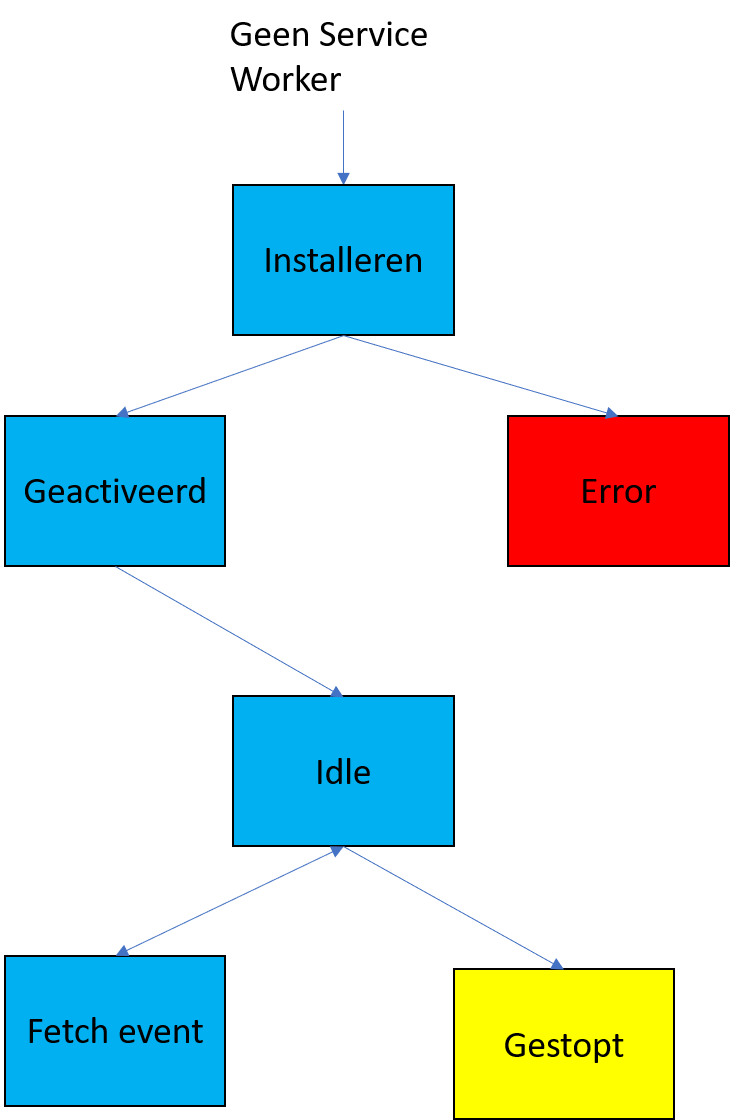
\includegraphics[scale=0.5]{img/lifeCycle.png}
	
	Voordat de service worker kan geïnstalleerd worden moeten we deze eerst registreren.
	
\begin{lstlisting}
if ('serviceWorker' in navigator) {
window.addEventListener('load', function() {
navigator.serviceWorker.register('/sw.js').then(function(registration) {
// Registration was successful
console.log('ServiceWorker registration successful with scope: ', registration.scope);
}, function(err) {
// registration failed :(
console.log('ServiceWorker registration failed: ', err);
});
});
}
\end{lstlisting}

Als je je service worker geregistreerd hebt, zal de browser deze direct installeren op de achtergrond. Je kan vanaf nu ook je service worker bekijken in de developer tools van Chrome (zie figuur \ref{fig:swDev}).

Tijdens het installeren kan je in het script meegeven wat het moet doen. In de meeste gevallen zal hier ook het cachen van statiche bestanden gebeuren. Aangezien deze statisch zijn en weinig veranderingen nodig hebben hoeft dit eenmalig te gebeuren, tijdens de installatie. Als bestanden niet kunnen gecached worden dan zal de installatiestap falen en zal deze nooit geactiveerd worden. De volgende keer zal de browser opnieuw proberen de service worker te installeren.
\begin{lstlisting}
var CACHE_NAME = 'my-site-cache-v1';
var urlsToCache = [
'/',
'/styles/main.css',
'/script/main.js'
];

self.addEventListener('install', function(event) {
// Perform install steps
event.waitUntil(
caches.open(CACHE_NAME)
.then(function(cache) {
console.log('Opened cache');
return cache.addAll(urlsToCache);
})
);
});
\end{lstlisting}


Nadat de service worker geïnstalleerd is wordt deze geactiveerd. Dit is de ideale plaats om oude caches te verwijderen en te zorgen dat de data die wel bewaard wordt up to date is.

\subsection{Application shell}
De application of app shell is het minimum aan HTML, CSS en Javascript dat je nodig hebt om je applicatie te kunnen tonen. Dit minimum wordt gecached zodat dit zelfs zonder internetverbinding altijd snel getoond kan worden aan de gebruiker. Hierdoor hoeft enkel de dynamische inhoud zoals een artikel geladen te worden via het netwerk.
De app shell is heel handig om al iets te kunnen tonen aan de gebruiker terwijl andere delen nog tijd nodig hebben om te laden.
\begin{figure}[h]
	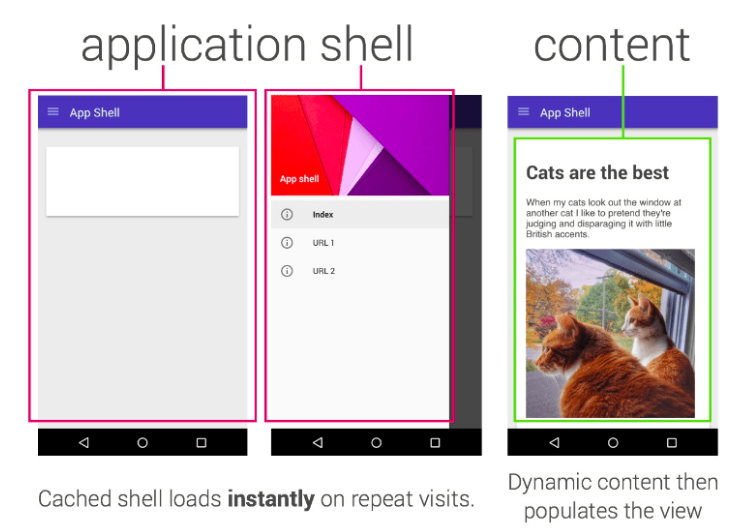
\includegraphics[scale=0.5]{img/appShell.png}
	\caption{Application shell}
	\label{fig:appShell}
\end{figure}
Zoals je op afbeelding \ref{fig:appShell} ziet, heb je in de application shell het minimum dat je wil tonen aan de gebruiker. Wanneer je de app ook bezoekt, zal dit altijd hetzelfde zijn. Aangezien hier weinig of geen verandering is, kan je dit lokaal opslaan (cachen). Het dynamisch gedeelte, het artikel, wordt wel via het netwerk geladen. Dit gedeelte, de inhoud, is niet altijd hetzelfde en zal vaak veranderen. Het is dus niet nodig dit lokaal op te slaan. Als er toch updates aan bestanden van de app shell worden gedaan, zal de progressive web app dit zien. De volgende keer dat de gebruiker online is, zal de app de oude bestanden vervangen door de nieuwe. Als ontwikkelaar is het belangrijk op voorhand te kijken welke bestanden je gaat cachen en welke niet.
Belangrijke voorwaarden voor de app shell zijn: 
\begin{itemize}  
	\item Snel laden
	\item Zo weinig mogelijk data gebruiken
	\item Statische bestanden gebruiken van de lokale cache
	\item Inhoud en navigatie scheiden
\end{itemize}

Dit is een voorbeeld van een app shell waarbij het sw.js bestand wordt gecachet. 
\lstdefinelanguage{JavaScript}{
	morekeywords={typeof, new, true, false, catch, function, return, null, catch, switch, var, if, in, while, do, else, case, break},
	morecomment=[s]{/*}{*/},
	morecomment=[l]//,
	morestring=[b]",
	morestring=[b]'
}
\lstdefinelanguage{HTML5}{
	language=html,
	sensitive=true, 
	alsoletter={<>=-},
	otherkeywords={
		% HTML tags
		<html>, <head>, <title>, </title>, <meta, />, </head>, <body>,
		<canvas, \/canvas>, <script>, </script>, </body>, </html>, <!, html>, <style>, </style>, ><
	},  
	ndkeywords={
		% General
		=,
		% HTML attributes
		charset=, id=, width=, height=,
		% CSS properties
		border:, transform:, -moz-transform:, transition-duration:, transition-property:, transition-timing-function:
	},  
	morecomment=[s]{<!--}{-->},
	tag=[s]
}


\begin{lstlisting}
<!DOCTYPE html>
<html>
<head>
<meta charset="utf-8">
<title>App Shell</title>
<link rel="manifest" href="/manifest.json">
<meta http-equiv="X-UA-Compatible" content="IE=edge">
<meta name="viewport" content="width=device-width, initial-scale=1.0">
<link rel="stylesheet" type="text/css" href="styles/inline.css">
</head>

<body>
<header class="header">
<h1 class="header__title">App Shell</h1>
</header>

<nav class="nav"></nav>

<main class="main"></main>

<div class="dialog-container"></div>

<div class="loader">
<!-- Show a spinner or placeholders for content -->
</div>

<script src="app.js" async></script>
<script>
if ('serviceWorker' in navigator) {
navigator.serviceWorker.register('/sw.js').then(function(registration) {
// Registration was successful
console.log('ServiceWorker registration successful with scope: ', registration.scope);
}).catch(function(err) {
// registration failed :(
console.log('ServiceWorker registration failed: ', err);
});
}
</script>
</body>
</html>
\end{lstlisting}


Na het creëren van je progressive web app, kan je deze laten auditeren door lighthouse. Je progressive web app krijgt een rapport speciaal voor jou opgemaakt. Je krijgt hier een score (op 100) op verschillende punten). Het rapport toont ook waar je nog dingen kunt verbeteren.


	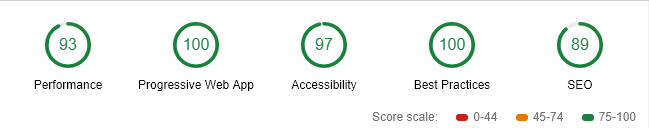
\includegraphics[scale=1]{img/audit.png}


\begin{itemize}  
	\item Performance: Dit toont hoe goed je huidige app presteert. Dit zal onder andere meten hoe snel de pagina laad.
	\item Progressive web app: In welke mate voldoet de app aan de checklist waaraan een progressive web app moet voldoen. Dit gaat ondere andere kijken of er een pictogram is voor het hoofdscherm van een telefoon.
	\item Accessibility: Hoe toegankelijk is je app. Hier kan je een goede score krijgen door onder andere een goed kleurencontrast te gebruiken op je webpagina's.
	\item Best practices: Hou je je aan de best practices omtrent het schrijven van een web app. Hier wordt er onder andere gekeken of je geen error logs in de consoles toont.
	\item SEO: Is je pagina optimaal voor zoekmachines?
\end{itemize}



%% Voeg hier je eigen hoofdstukken toe die de ``corpus'' van je bachelorproef
%% vormen. De structuur en titels hangen af van je eigen onderzoek. Je kan bv.
%% elke fase in je onderzoek in een apart hoofdstuk bespreken.

%\input{}
%\input{}
%...

%%=============================================================================
%% Conclusie
%%=============================================================================

\chapter{Conclusie}
\label{ch:conclusie}

%% TODO: Trek een duidelijke conclusie, in de vorm van een antwoord op de
%% onderzoeksvra(a)g(en). Wat was jouw bijdrage aan het onderzoeksdomein en
%% hoe biedt dit meerwaarde aan het vakgebied/doelgroep? Reflecteer kritisch
%% over het resultaat. Had je deze uitkomst verwacht? Zijn er zaken die nog
%% niet duidelijk zijn? Heeft het onderzoek geleid tot nieuwe vragen die
%% uitnodigen tot verder onderzoek?

 




%%---------- Back matter ------------------------------------------------------

\printbibliography
\addcontentsline{toc}{chapter}{\textcolor{maincolor}{\IfLanguageName{dutch}{Bibliografie}{Bibliography}}}


\listoffigures
\listoftables

\end{document}
